%! Author = Frederik Bußmann
%! Date = 22.06.2023

\section{Entwicklung der CI-Strategie} \label{sec:04-implementation}

Im folgenden wird die konzipierte \acrshort{ci}-Strategie des vorherigen Kapitels praktisch umgesetzt.
Zunächst wird eine Projektumgebung geschaffen, in der die geplanten \acrshort{ci}-Tools und eine Shopware-Instanz zum
Testen installiert werden.
Daraufhin werden die installierten Tools für das Testen des lokal aufgesetzten Shops konfiguriert und angepasst,
wobei der Code eines eigens dafür angelegten Beispiel-Plugins als Test-Grundlage verwendet wird.
Anschließend werden verschiedene Deployment-Umgebungen für das Testen des Shops angelegt und für diese Umgebungen
automatisierte Deployment-Konfigurationen zum Ausliefern durch die zu entwickelnden Pipelines erstellt.
Zuletzt werden anhand der konfigurierten Tools und dem Beispiel-Shop die eigentlichen Pipelines zum
automatisierten Bauen, Testen und Ausliefern von Shopware-Projekten erstellt.

\subsection{Aufsetzen der Projektumgebung} \label{subsec:04-implementation-1}

Für das Implementieren der konzipierten Strategie muss zunächst eine lokale Entwicklungsumgebung bestehen, in der ein
Shopware-Projekt und die geplanten \acrshort{ci}-Tools installiert werden können.
Hierbei wurde sich für die Nutzung des von Shopware gestellten Docker-Containers entschieden, welcher die
Abhängigkeiten für das Betreiben der Plattform gesammelt bereitstellt.\footpartcite{shopware-docker}
Das Ausführen der Shop-Software ohne Docker ist dabei weiterhin möglich, indem dessen Abhängigkeiten direkt auf dem
Entwicklungssystem installiert werden.
Zunächst wurde ein Ordner für die Shopware-Installation angelegt und Package-Konfigurationen für Composer und NPM
erstellt.
In der Composer-Konfigurations-Datei\ \shellinline{composer.json} werden die Pakete für die PHP-basierten
\acrshort{ci}-Tools PHPUnit, Infection,\ \acrshort{phpcs},\ \acrshort{phpmd}, PHPStan, Deptrac und License Checker
verwaltet.
Die Paket-Abhängigkeiten für die JavaScript-basierten Tools Eslint, Jest, Cypress und Danger JS werden in der
Konfigurations-Datei\ \shellinline{package.json} hinterlegt.
In den beiden Konfigurations-Dateien wurden zunächst lediglich der Projekt-Titel, Autoren und die Version und die Art
der Lizenz des Projekts definiert.
Um die Software bei der Entwicklung zwischenspeichern und fehlerhafte Änderungen zurückrollen zu können,
wurde an dieser Stelle bereits ein\ \acrshort{vcs} eingeführt.
Hierbei wurde sich für GitLab entschieden, da das zur Konzipierung der Strategie genutzte GitLab CI/CD bereits in der
Versionsverwaltung integriert ist.
\\\\
Bevor der Beispiel-Shop im Shopware-Verzeichnis aufgesetzt werden kann, muss zunächst die geplante Docker-Umgebung
definiert werden.
Docker bietet hierfür ein eingebautes Plugin namens\ \glqq Docker Compose\grqq, welches die Konfiguration von
verschiedenen Containern in \acrshort{yaml}-Dateien ermöglicht.
Dies hat den Vorteil, dass verschiedene Services wie der Shop-Container selbst, die SQL-Datenbank für den Betrieb des
Shops und weitere Dienste wie Message Queue, Search Engine und Caches gesammelt konfiguriert und mit einem einzigen
Befehl angelegt werden können.
Für den Betrieb des Shops wurde also zunächst die Datei\ \shellinline{docker-compose.yml} erstellt und die
Container-Konfigurationen für das Shopware-Image und eine MySQL-Instanz angelegt.
Das Docker-Image\ \shellinline{shopware/development} wird hierzu mit dem Tag\ \shellinline{8.2-composer-2} hinterlegt,
sodass der daraus resultierende Shopware-Container PHP in Version 8.2 und Composer in Version 2 zur Verfügung stellt.
Um den Quellcode der zu betreibenden Shop-Software in den Container laden zu können, wird das Shopware-Verzeichnis als
Volume in den Container eingebunden.
Dies ermöglicht, dass Änderungen am Quellcode, die auf dem Host-System vorgenommen werden, direkt im Container sichtbar
sind und umgekehrt.
Hierfür wird in der Datei\ \shellinline{docker-compose.yml} unter dem Schlüssel\ \shellinline{volumes} der Pfad zum
lokalen Shopware-Verzeichnis und der entsprechende Pfad im Container angegeben, in diesem Fall der Order
\shellinline{/app}.
Zusätzlich wird der Port\ \shellinline{80} des Shopware-Containers auf den entsprechenden Port des Host-Systems
weitergeleitet, wodurch der Zugriff auf den Shop über einen Webbrowser ermöglicht wird.
Die MySQL-Instanz wird über das offizielle MySQL-Image\ \shellinline{mysql} in der Version 8 bereitgestellt.
\footpartcite{mysql-image}
Ein Docker Volume wird für das Datenverzeichnis der MySQL-Instanz hinterlegt, um Datenverlust beim Wechseln der Version
oder dem Herunterfahren des Containers zu vermeiden.
Der Port\ \shellinline{3306} des MySQL-Containers wird dabei auch auf den entsprechenden Port des Host-Systems
weitergeleitet, um Zugriff auf die Datenbank zu ermöglichen.
Die Zugriffs-Informationen und Einstellungen können in der Form von Umgebungsvariablen in der
Compose-Konfiguration gespeichert werden.
Beide Container sind dabei Teil des gleichen Netzwerks, welches in der Konfigurations-Datei unter dem Schlüssel
\shellinline{networks} definiert ist.
Dies ermöglicht die Kommunikation zwischen den Containern über das interne Docker-Netzwerk.
Mit dieser Konfiguration ist es möglich, eine lokale Entwicklungsumgebung mit Docker aufzusetzen, die den Anforderungen
der meisten Shopware-Projekte gerecht wird.
Die vollständige Container-Konfiguration in der Datei\ \shellinline{docker-compose.yml} kann in Anhang
\ref{sec:appendix-1} eingesehen werden.
\\\\
Nach dem Aufsetzen der lokalen Entwicklungsumgebung und dem Bereitstellen der Abhängigkeiten von Shopware wurde der
Beispiel-Shop im \shellinline{shopware}-Verzeichnis installiert.
Hierzu wurde der Paket-Manager Composer genutzt, welcher den Befehl\ \shellinline{composer create-project} bereitstellt,
um verschiedene Software-Projekte zu erstellen.
Shopware pflegt eine eigene Vorlage zum Erstellen eines Shop-Projekts, welche unter dem Namen
\shellinline{shopware/production} durch den Create-Project-Befehl genutzt werden kann.
Anschließend kann der Service bereits im Webbrowser erreicht werden und die lokale Installation des Shops durch den
Web-basierten Shopware-Installer durchgeführt werden.
In diesem Schritt werden die Stammdaten des Shops festgelegt und die Datenbankverbindung mit dem zuvor angelegten
MySQL-Service hergestellt.
Anhand der hier angegebenen Daten erstellt die Software eine \shellinline{.env}-Datei, in der die Umgebungsvariablen
für die Verbindung mit der lokalen Datenbank gespeichert werden.

\begin{figure}[H]
    \centering
    
\includegraphics[width=\textwidth]{images/content/best-it-example-plugin}
    \captioncite[Eigene Darstellung]{}{Beispiel-Plugin zur Konfiguration der \acrshort{ci}-Tools}
    \label{fig:example-plugin}
\end{figure}

Um die geplante \acrshort{ci}-Strategie umsetzen zu können, muss neben der lokalen Shopware-Umgebung auch eigener
Quellcode existieren, welcher zur Konfiguration der Test- und Analyse-Tools genutzt werden kann.
Da die Strategie das Erweitern der Shopware-Platform durch eigens entwickelte Plugins abdecken soll, wurde zunächst ein
Beispiel-Plugin erstellt.
Hierzu wurde der Plugin-Ordner\ \shellinline{BestItExamplePlugin} im Verzeichnis \shellinline{custom/static-plugins}
der Shopware-Installation angelegt.
Die Konfiguration des Plugins erfolgt dabei über den Paket-Manager Composer, wobei eine eigene
Konfigurations-Datei\ \shellinline{composer.json} im Plugin-Ordner angelegt wird.
Hier werden Grund-Informationen über das Plugin wie dessen Autor, Version, Abhängigkeiten und der Position des
Quellcodes im Plugin-Ordner definiert:

\jsonfile{code/plugin-composer.json}

Um sowohl testbaren PHP- als auch JavaScript-Code bereitzustellen, wurden jeweils eigene Code-Beispiele in beiden
Sprachen angelegt.
Für das Einführen und Konfigurieren der geplanten PHP-basierten \acrshort{ci}-Tools wurden zunächst ein
Beispiel-Controller und ein Beispiel-Service angelegt.
Der Controller befindet sich im Unter-Verzeichnis\ \shellinline{src/Controller} des Plugin-Ordners und wird durch das
Öffnen der Route\ \shellinline{http://localhost/example} im Webbrowser aufgerufen.
Der Controller ruft hierbei den Beispiel-Service auf, welcher eine Berechnung durchführt und diese anschließend zurück
an den Controller übergibt, sodass das Ergebnis im Frontend ausgegeben werden kann.
Die Konfiguration der Controller und Services wird innerhalb eines Shopware-Plugins über die Datei
\shellinline{services.xml} im Ordner\ \shellinline{src/Resources/config} des Plugin-Verzeichnisses gesteuert.
Für das Konfigurieren der JavaScript-Tools der Strategie wurde innerhalb des Beispiel-Plugins eigener
JavaScript-Code eingeführt.
Die JavaScript-Erweiterung nutzt wie auch der zuvor definierte PHP-Code einen eigenen Beispiel-Service, welcher eine
Berechnung durchführt, und diese an die aufrufende Skript-Instanz zurückgibt.
Um das Skript inklusive des Services in die Shopware-Storefront einzubinden, wurde die Datei\ \shellinline{main.js} im
Verzeichnis\ \shellinline{src/Resources/app/storefront/src} verwendet, welche für das Laden von
JavaScript-Abhängigkeiten durch die Software automatisch referenziert wird.
Das Beispiel-Plugin bietet somit eine Grundlage zum Analysieren von JavaScript- und PHP-Code und ermöglicht das Anlegen
von Tests für die eingeführte Logik, wodurch die geplanten Testing-Tools konfiguriert und auf ihre Funktion geprüft
werden können.
In Abbildung\ \ref{fig:example-plugin} wird ein Screenshot aus dem Shopware-Backend aufgezeigt, in welchem das
installierte und aktivierte Beispiel-Plugin zu sehen ist.

\subsection{Konfiguration der Testing- und QA-Tools} \label{subsec:04-implementation-2}

Um die geplanten \acrshort{ci}-Tools für das automatisierte Prüfen des im Projekt eingeführten PHP- und JavaScript-Codes
installieren zu können, muss die Umgebung in der diese ausgeführt werden, an die Umgebung des Shops angeglichen werden.
Hierbei könnte zunächst der Ordner mit den Paket-Manager- und Tool-Konfigurationen in den bestehenden Shopware-Container
eingebunden werden.
Da das Ausführen der geplanten Tools im späteren Pipeline-Umfeld jeweils isoliert in einem eigenen Container und
parallel ausführt wird, wurde sich allerdings für eine eigene Container-Instanz als Tool-Umgebung entschieden.
Um einen Container im Hauptverzeichnis des Projekts zu starten, welcher die Abhängigkeiten der Shopware-Platform
bietet, kann weiterhin das von Shopware gestellte Development-Image lokal genutzt werden:
\\\\
\shellinline{docker run -it -v ".:/app" shopware/development:8.2-composer-2 /bin/bash}
\\\\
Durch diesen Konsolenbefehl wird eine Instanz des Development-Images gestartet, welche das aktuelle Verzeichnis in den
Ordner\ \shellinline{/app} einbindet.
Der Befehl nutzt dabei das Argument\ \shellinline{-v}, um ein Volume vom Host-System zum Container zu schaffen, welches
die spezifizierten Ordner-Pfade miteinander verbindet.
Die Argumente\ \shellinline{-i} und\ \shellinline{-t} sorgen dabei für das interaktive Starten des Containers im
\acrshort{tty}-Modus, wodurch ein Terminal bereitgestellt wird.
Durch das Angeben der ausführbaren Datei\ \shellinline{/bin/bash} am Ende des Befehls wird nach dem Starten des
Containers ein Bash-Terminal ausgeführt.
In diesem Terminal stehen anschließend die benötigten Abhängigkeiten für das Installieren und Ausführen der
\acrshort{ci}-Tools und Shopware bereit.
Nachfolgend werden die geplanten \acrshort{ci}-Tools für das automatisierte Prüfen des im Shopware-Projekt eingeführten
PHP- und JavaScript-Codes installiert und konfiguriert:

\subsubsection{PHPUnit}

% @TODO: \footpartcite{xdebug} für Coverage in Text einbauen

Das Testing-Framework PHPUnit wird als Entwicklungs-Abhängigkeit mit dem Paket-Namen\ \shellinline{phpunit/phpunit}
in der Datei\ \shellinline{composer.json} installiert.
Durch das Framework ist es möglich, eigene Unit-Tests in Form von PHP-Klassen und Funktionen in einem Shopware-Plugin
anzulegen.
Anschließend wurde für das Erstellen von Unit-Tests im Beispiel-Plugin die Verzeichnisse\ \shellinline{Tests} und
\shellinline{Tests/Unit} angelegt, in welchem die PHP-Klassen der Tests abgelegt werden.
Um die in diesem Ordner befindlichen Tests ausführen zu können, muss das Verzeichnis in der
Composer-Konfigurations-Datei des Plugins referenziert werden:

\jsonfile{code/phpunit-composer.json}

Anschließend wurde für die Konfiguration des Test-Frameworks die Datei\ \shellinline{phpunit.xml.dist} angelegt.
In dieser Datei werden Einstellungen für die Position der Test-Dateien und auszuschließenden Dateien, die
Erzeugung von Auswertungen zur Test-Abdeckung, dem Erstellen von Log-Dateien und dem Definieren des Cache-Verzeichnisses
für durchgeführte Tests vorgenommen.
Nach dem Erstellen der Datei wurden zum Prüfen der Konfiguration Unit-Tests für das Beispiel-Plugin kreiert.
Die Namenskonvention von Unit-Tests wurde für die \acrshort{ci}-Strategie als Name der zu testenden Klasse mit dem
Suffix\ \glqq Test\grqq\ festgelegt.
Zunächst wurde ein Unit-Test für die Datei\ \shellinline{src/BestItExamplePlugin.php} angelegt, welche das Nutzen des
Plugins in Shopware ermöglicht.
Dieser Test prüft zunächst nur, ob die zu testende Klasse existiert und erfolgreich instanziiert werden kann:

\phpfile{code/BestItExamplePluginTest.php}

% @TODO: Text verlängern, verbessern und Bild evtl. weglassen oder austauschen

Der Test erweitert hierbei die von PHPUnit gegebene Klasse\ \shellinline{TestCase} und nutzt zum Vergleichen der
erwarteten und der tatsächlichen Ergebnisse von aufgerufenen Funktionen verschiedene statische Funktionen des
Frameworks.
Neben dem Test der Plugin-Klasse wurde ein weiterer Test für den Beispiel-Service angelegt.
Die Tests können innerhalb des \acrshort{ci}-Containers anschließend mit dem Befehl
\shellinline{vendor/bin/phpunit} aufgerufen werden.
In Abbildung\ \ref{fig:phpunit-results} wird ein Terminal aufgezeigt, in dem PHPUnit-Tests durchgeführt werden.
Hierbei generiert das Framework auch Informationen zur Test-Abdeckung:

\begin{figure}[H]
    \centering
    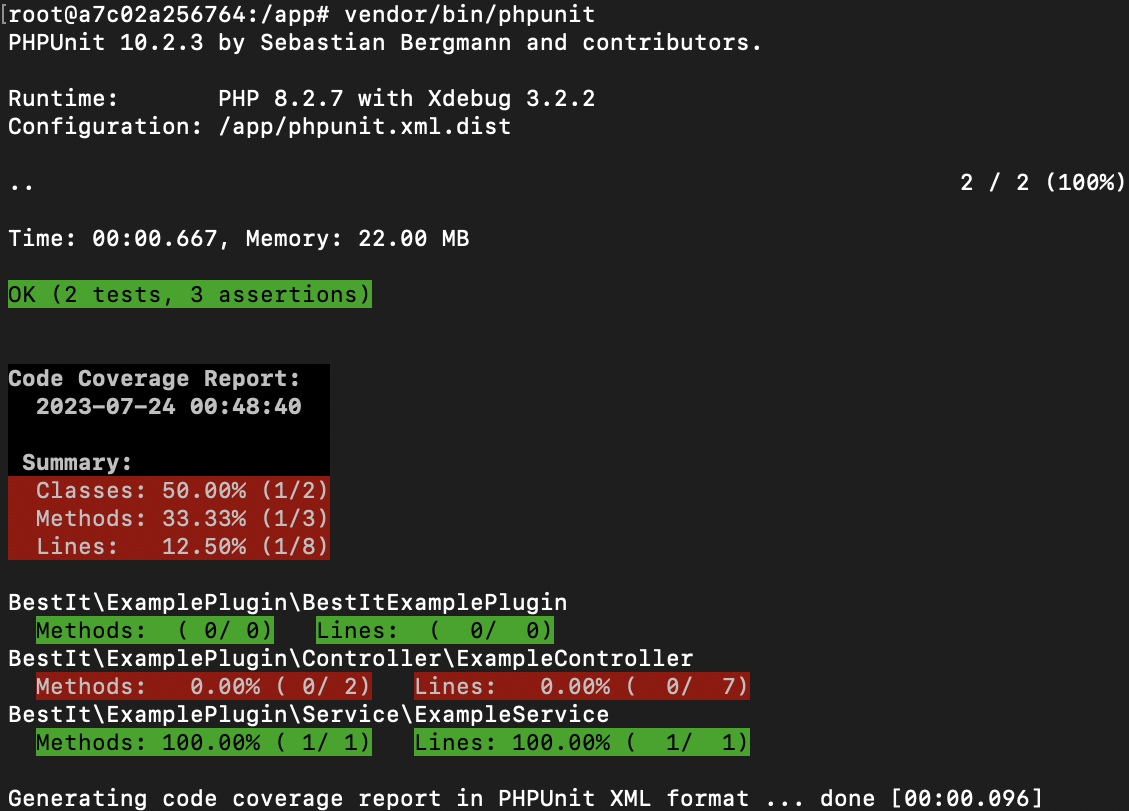
\includegraphics[width=0.6\textwidth]{images/content/phpunit-result}
    \captioncite[Eigene Darstellung]{}{Ergebnisse der PHPUnit-Tests inklusive Code-Coverage}
    \label{fig:phpunit-results}
\end{figure}

\subsubsection{Infection}

Das Mutation-Testing-Framework Infection wird, wie auch PHPUnit, in der Konfigurations-Datei
\shellinline{composer.json} des Projekts installiert.
Nach der Installation des Pakets durch Composer unter dem Namen\ \shellinline{infection/infection} steht das Tool zum
Ausführen von Mutation-Tests bereit.
Das Programm verändert dabei den Quellcode des zu testenden Projekts und führt anschließend PHPUnit aus, wobei
geprüft wird, welche Änderungen durch die gegebenen Tests unbemerkt blieben.
Da für das Projekt bereits Tests angelegt wurden, musste Infection lediglich für die Prüfung der bestehenden
Test-Suite konfiguriert werden.
Hierzu wurden im Hauptverzeichnis des Projekts zwei Dateien angelegt:\ \shellinline{infection.json} und
\shellinline{infection-bootstrap.php}.

% @TODO: infection.json und infection-bootstrap.php erklären

\subsection{Deployments und Umgebungen} \label{subsec:04-implementation-3}

% Hosting von Servern für Shopware-Umgebungen zum Testen aufsetzen + das Tool Deployer implementieren

\subsection{Implementierung der Pipelines} \label{subsec:04-implementation-4}

% Pipelines erstellen und konfigurieren

\clearpage
